\section{Algorithm}
\label{sec:algorithm}

In this section, we first introduce Graph Fourier Transform concept, explaining eigenvector and eigenvalue meanings, then based on that define anomaly index of graph. The next is to describe graph wavelet's features such as reconstruction and localization. In section~\ref{sec:Group_Anomaly_Detection_via_graph_wavelet}, we propose the group anomaly detection algorithm via graph wavelet. And in section~\ref{sec:Group Absenteeism Event Detection} we present the two-pass event detection algorithm.

\subsection{Graph Fourier Transform}
\label{sec:Graph_Fourier_Transform}
Given a signal $f$ defined on graph $\mathbf{G}$, its Graph Fourier Transform is considered as the projection of $f$ on the complete set of $\{\chi_l\}_{l=0}^{N-1}$, and is written as~\cite{hammond2011wavelets}:
\begin{equation}
\label{eq:Graph_Fourier_Transform1}
\hat{f}(l)=<\chi_{l},f>=\sum_{i=1}^{N}\chi^*_{l}(i)f(i)
\end{equation}
Since $\{\chi_l\}_{l=0}^{N-1}$ is complete, therefore, $f$ can be recovered by its Graph Fourier Transform coefficients $\hat{f}(l)$ as~\cite{hammond2011wavelets}:
\begin{equation}
\label{eq:Inverser_Graph_Fourier_Transform}
f(n)=\sum_{l=0}^{N-1}\hat{f}(l)\chi_{l}(n)
\end{equation}
$\hat{f}(l)$ is the coefficient of component $\chi_l$.


\begin{figure}[h]
	\centering
    {
		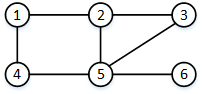
\includegraphics[height=1.4in] {figures/graph_G.png}
	}
	\caption{Graph $\mathbf{G_1}$, all edges's weight are $1$.}
	\label{fig:graph_G}
\end{figure}


\begin{figure}[ht]
	\centering
	\subfigure[]{
		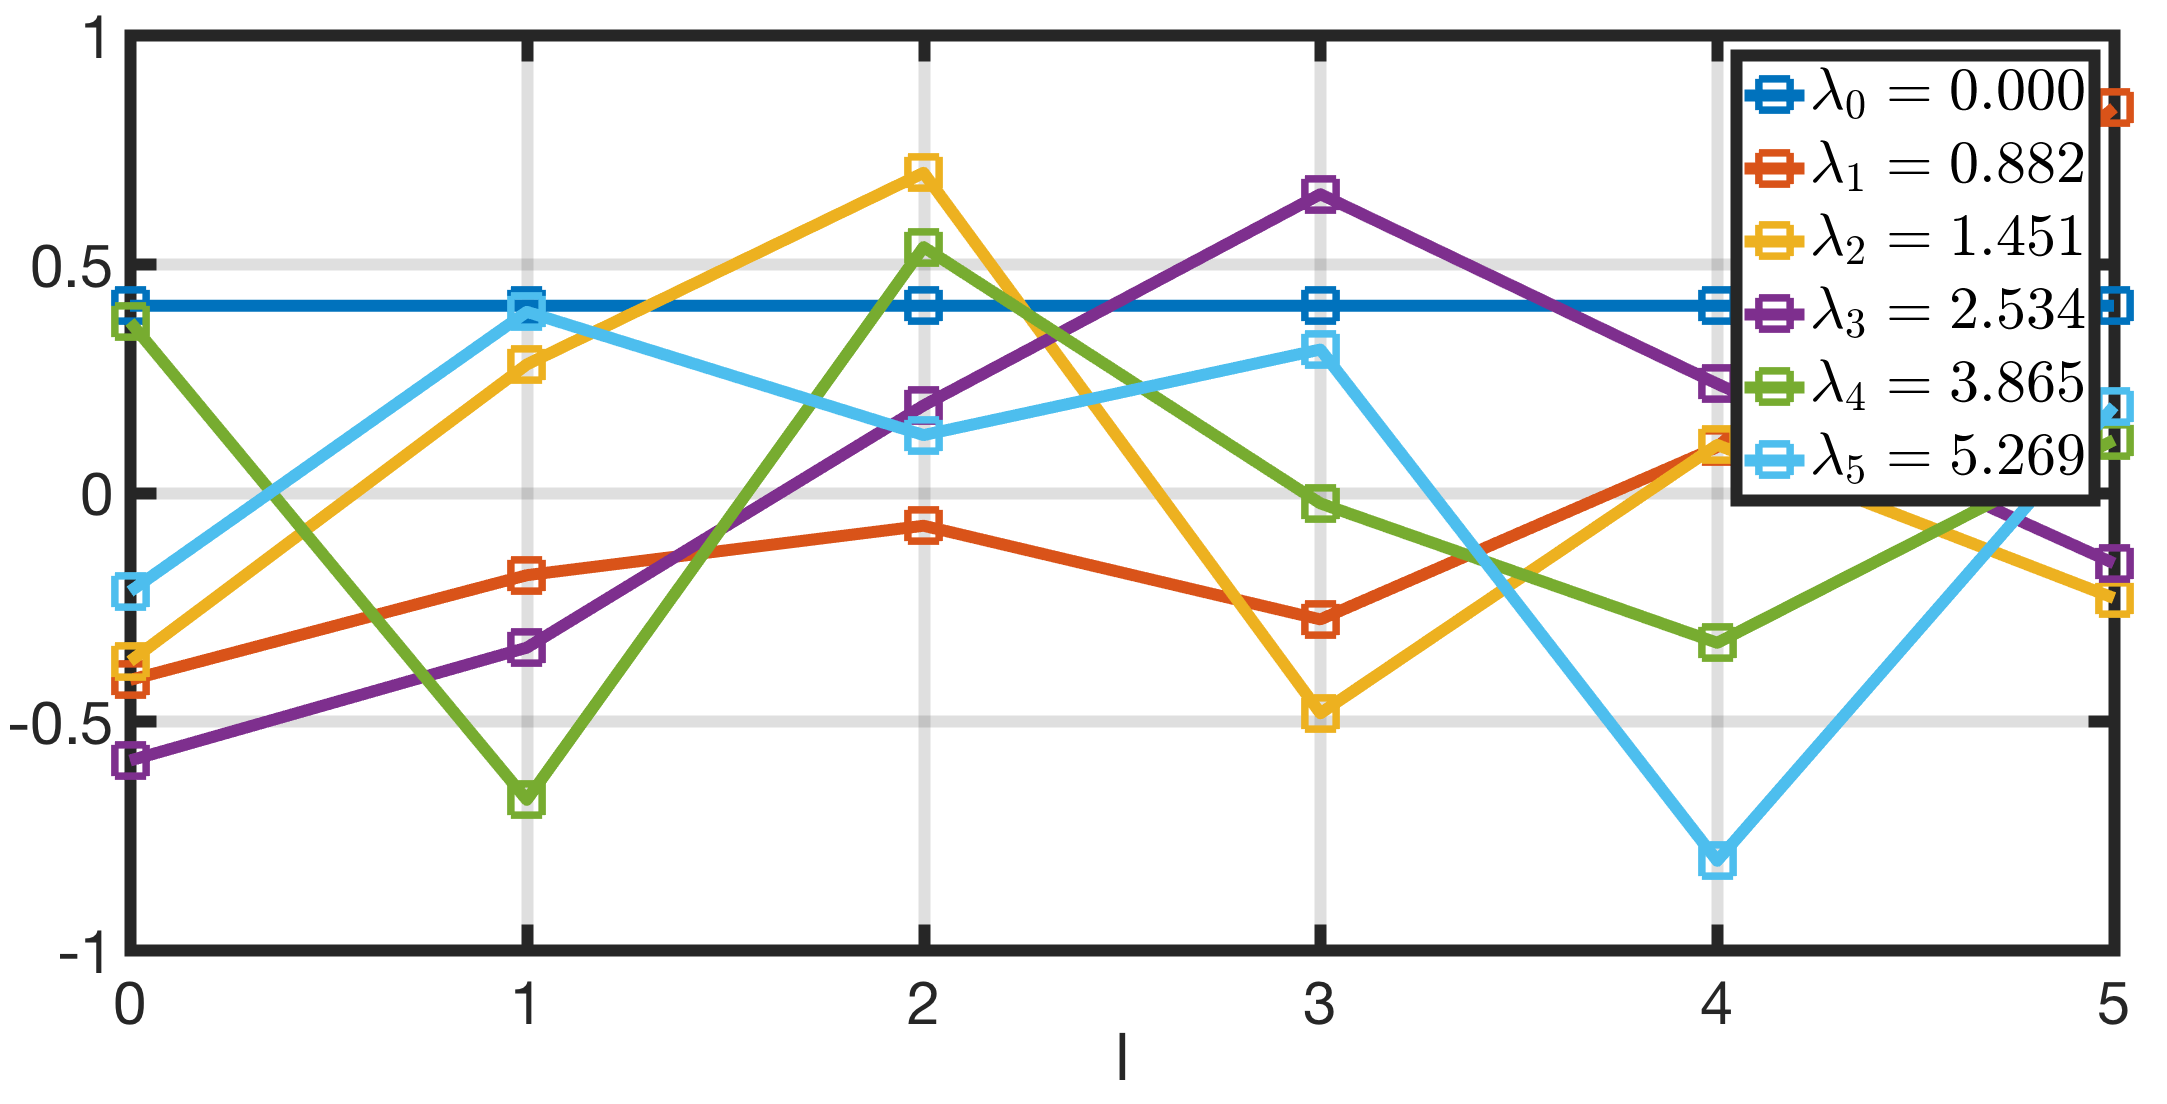
\includegraphics[width= 3in, height=1.6in] {figures/frequency.png}
		\label{fig:frequency1}
	}
	\subfigure[]{
		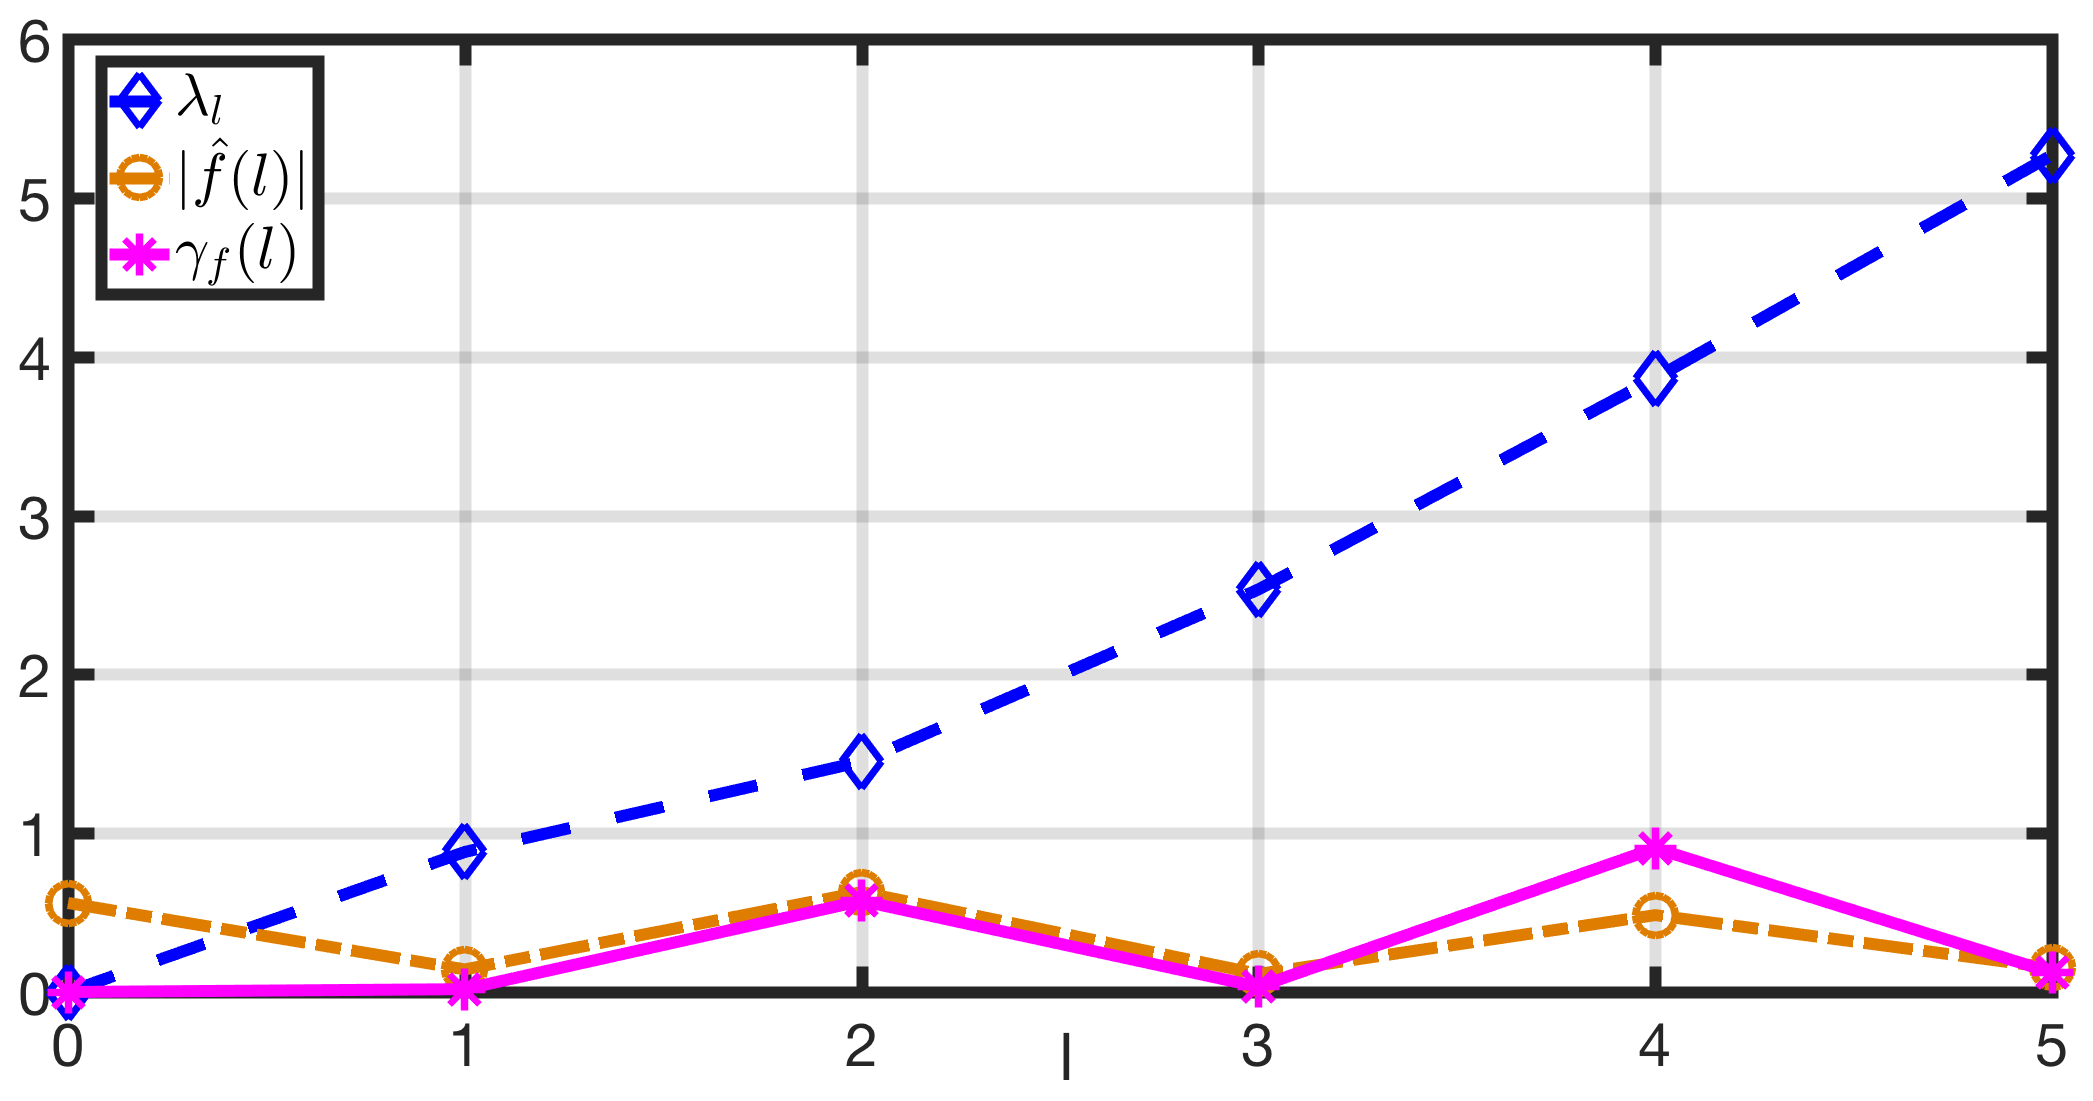
\includegraphics[width= 2.8in, height=1.6in] {figures/g1_gamma.png}
		\label{fig:g1_gamma}
	}

	\subfigure[]{
		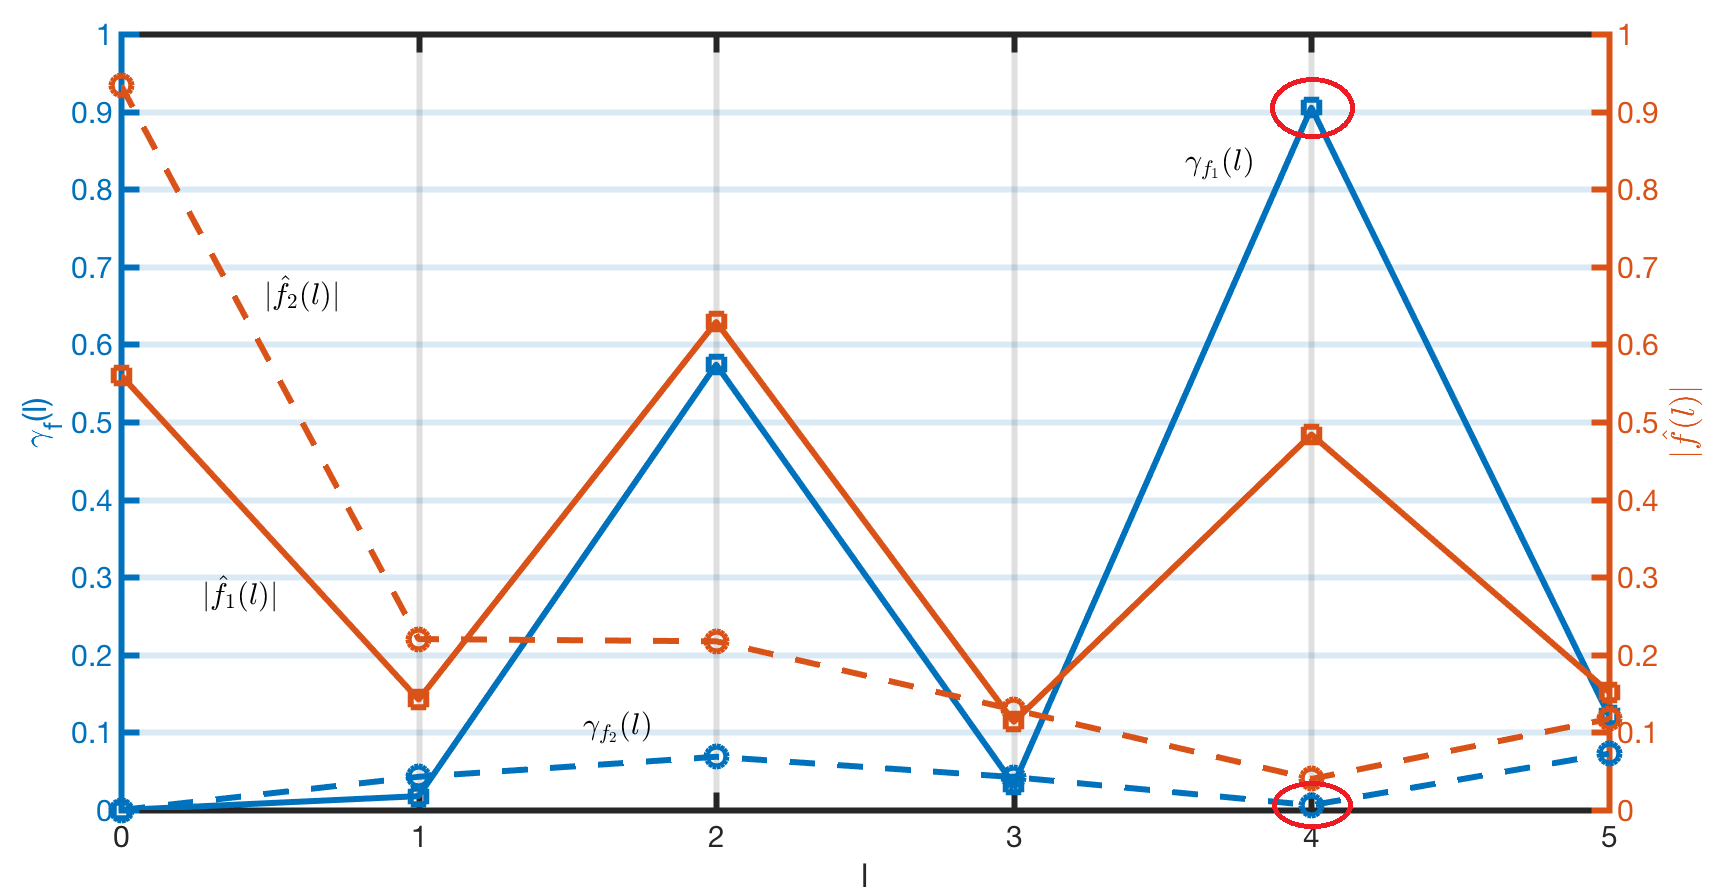
\includegraphics[width= 3in] {figures/same_graph.png}
		\label{fig:same_graph}
	}

	\caption{(a): Eigenvector distribution along each vertex in graphs $\mathbf{G_1}$.  (b): anomaly index $\gamma_f(l)$ of $f_1=[2,3,4,3,2,1]$ on graph $\mathbf{G_1}$. (c): anomaly index $\gamma_f(l)$ of $f_1=[2,3,4,3,2,1]$  and $f_2=[2,2,-3,4,3,1]$ on graph $\mathbf{G_1}$, where $\gamma_{f_1}=0.905$, and $\gamma_{f_1}=0.073$, labelled in red oval.}
	\label{fig:f_on_g2}
\end{figure}


\subsubsection{eigenvector $\chi_l$}
As an analog with classical signal processing, eigenvector $\chi_l$ is also called frequency of $\mathbf{G}$ by some researchers. In the later part of this paper, $\chi_l$ will be called eigenvector or frequency, alternatively. However, unlike the traditional frequency concept in classical signal processing fields, the frequencies of $\mathbf{G}$ is a set of discreet vectors with length of $|V|$. Interestingly, like the classical signal Fourier Transform, Parseval relation still holds; i.e.~\cite{shuman2015vertex},
\begin{equation}
\label{eq:Parseval}
||\hat{f}||_2^2=||f||_2^2
\end{equation}
Equation~\ref{eq:eigenvalues} means that energy in vertex domain and frequency domain is equal for any graph signal $f$. Without loss of generality, we assume $||f||_2 =1$, if there is no explicit notations.

\subsubsection{eigenvalue $\lambda_l$}
According to the definition of eigenvalue $\lambda_l$  in Equation~\ref{eq:eigenvalues}, the following equation holds:
\begin{equation}
\label{eq:lambda1}
\chi_{l}^T\lambda_{l}\chi_{l}=\chi_{l}^T\mathcal{L}\chi_{l}= \sum_{e_{mn}\in E} w_
{mn}[\chi_{l}(m)-\chi_{l}(n)]^2
\end{equation}Since $\chi_{l}$ is normalized, and $||\chi_{l}||_2 =1$, then,
\begin{equation}
\label{eq:lambda2}
\chi_{l}^T\lambda_{l}\chi_{l}=\lambda_l= \sum_{e_{mn}\in E} w_
{mn}[\chi_{l}(m)-\chi_{l}(n)]^2
\end{equation}
From equation~\ref{eq:lambda2}, we can see that $\lambda_l$ summarizes all the eigenvector deviations on any directly connected vertices $v_m$ and $v_n$ in $\mathbf{G}$. Since each term in the summation of the right-hand side is non-negative, the eigenvectors associated with smaller eigenvalues are smoother; i.e., the component differences between neighboring vertices are
small~\cite{shuman2015vertex}. As the eigenvalue increases, larger differences in neighboring
components of the graph Laplacian eigenvectors is present.
Hence, for larger $\lambda_l$, its corresponding eigenvector, $\chi_l(n)$, has larger deviation among connected vertices. According to the definition of Laplacian matrix $\mathcal{L}$, it is easy to verify that $\lambda_0=0$ since $\mathcal{L}\cdot\vec{\textbf{1}}= 0\cdot\vec{\textbf{1}}$, where $\vec{\textbf{1}}=\{1,1,1,...,1\}$, and $\chi_o(n)=\frac{\vec{\textbf{1}}}{\sqrt{N}}$. Thus, $\chi_o(n)=\frac{\vec{\textbf{1}}}{\sqrt{N}}$, means $\chi_o(n)$ is constant on each vertex, and there is no deviation among any two vertices in $\chi_0(n)$. For this reason, $\chi_0(n)$ is considered as the least abnormal component of $\mathbf{G}$. Similarly, $\chi_{N-1}(n)$ is considered the most abnormal component of $\mathbf{G}$.

Fig \ref{fig:graph_G} shows an undirected graph $\mathbf{G_1}$, and each edge's weight is $1$. Fig \ref{fig:frequency1} shows  $\mathbf{G_1}$'s six eigenvectors distributions along each vertex. We can see, $\chi_0(l)$ is constant on very vertex, and has the smallest deviations along each edge. $\chi_5$ has the largest deviations, and the difference of $\chi_5(l)$ along each edge is larger than any other eigenvector on average.



\begin{figure}[t]
	\centering
	\subfigure[]{
		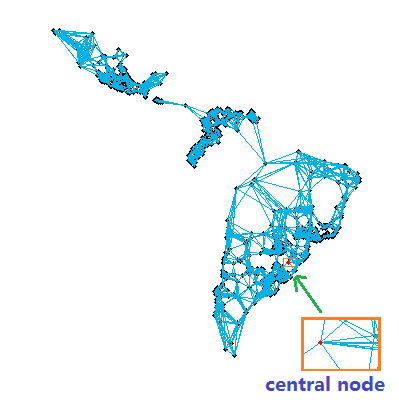
\includegraphics[height=1.6in] {figures/All-0.png}
		\label{fig:brazil1}
	}
	\subfigure[]{
		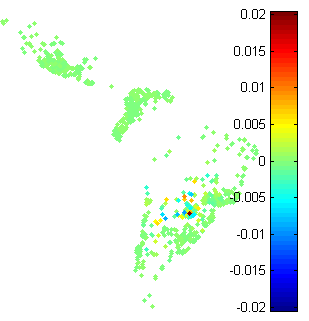
\includegraphics[height=1.6in] {figures/All-08.png}
		\label{fig:brazil2}
	}
		\subfigure[]{
		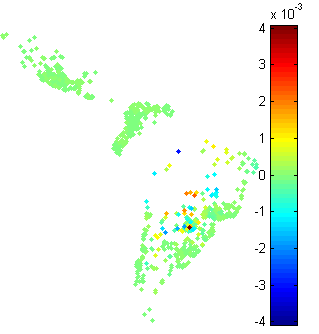
\includegraphics[height=1.6in] {figures/All-18.png}
		\label{fig:brazil3}
	}
	\subfigure[]{
		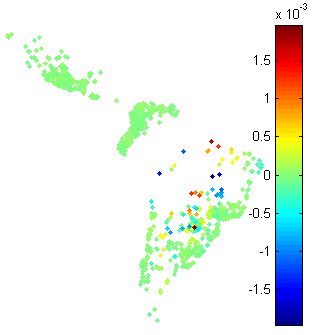
\includegraphics[height=1.6in] {figures/All-26.png}
		\label{fig:brazil4}
	}
    \subfigure[]{
		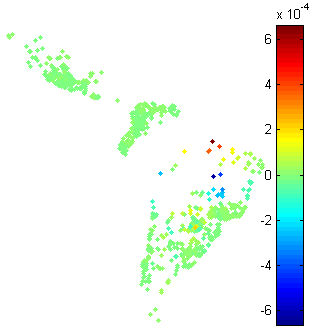
\includegraphics[height=1.6in] {figures/All-80.png}
		\label{fig:brazil5}
	}
	\subfigure[]{
		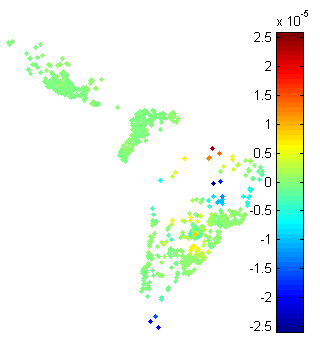
\includegraphics[height=1.6in] {figures/All-400.png}
		\label{fig:brazil6}
	}
	\caption{Spectral graph wavelet on South America. (a) vertex at which wavelets are centered in red dot. (b)-(f) wavelets, scales at 0.8, 1.8, 2.6, 8, and 40 respectively.}
	\label{fig:example2}
\end{figure}


\subsection{Global Anomaly Index}
\label{sec:signal_anomaly_on_Graph}

To quantify the anomaly of a vector $f$ defined on a graph $\mathbf{G}$, it's necessary to combine the intrinsic structures of $\mathbf{G}$ and $f$. As discussed above, $\hat{f}(l)$ represents the coefficient of frequency $\chi_l$, and $\hat{f}^2(l)$ is considered as the energy of frequency $\chi_l$. In addition, according to equation~\ref{eq:lambda2}, $\lambda_l$ represents the deviation of frequency $\chi_l$ along all the connected vertex. Therefore, in this paper, we define the anomaly Index of $\chi_l$ in $f$ as:
\begin{equation}
\label{eq:lambda3}
\gamma_f(l;\mathbf{G})=\lambda_l\hat{f}^2(l)= \lambda_l<f,\chi_l>^2
\end{equation}
$\gamma_f(l;\mathbf{G})$ depends on two parts, frequency $\chi_l$'s deviation sum $\lambda_l$, and its energy $\hat{f}^2(l)$. If the energy $\hat{f}^2(l)$ is small, even $\lambda_l$ is large, the anomaly Index of $\chi_l$ still might be small. Obviously, $\gamma_f(0;\mathbf{G})$ is always $0$ since $\lambda_0=0$. Further, we use the maximal value of $\gamma_f(l;\mathbf{G})$ to represent the global anomaly of $f$ on $\mathbf{G}$:
\begin{equation}
\label{eq:lambda4}
\gamma_f(\mathbf{G})=\underset{0 \leq l \leq N-1}{\max}{\gamma_f(l;\mathbf{G})}.
\end{equation}
Roughly speaking, $\gamma_f(l;\mathbf{G})$ means the anomaly extension of $\chi_l$ in $f$ defined on $\mathbf{G}$, in stead of meaning anomaly extension of vertex $v_l$.
For brevity, $\gamma_f(l;\mathbf{G})$  and $\gamma_f(\mathbf{G})$ are shortened as $\gamma_f(l)$ and $\gamma_f$, respectively, in some circumstance.


\begin{figure}[t]
	\centering
	\subfigure[$\mathbf{G_2}$]{
		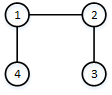
\includegraphics[height=1.1in] {figures/f_on_g1.png}
		\label{fig:scale1}
	}
	\subfigure[$\mathbf{G_3}$]{
		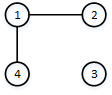
\includegraphics[height=1.1in] {figures/f_on_g2.png}
		\label{fig:scale2}
	}
	\caption{$f=[1,2,5,2]$ on two graphs $\mathbf{G_2}$ and $\mathbf{G_3}$.}
	\label{fig:f_on_g}
\end{figure}

\begin{figure}[t]
	\centering
    {
		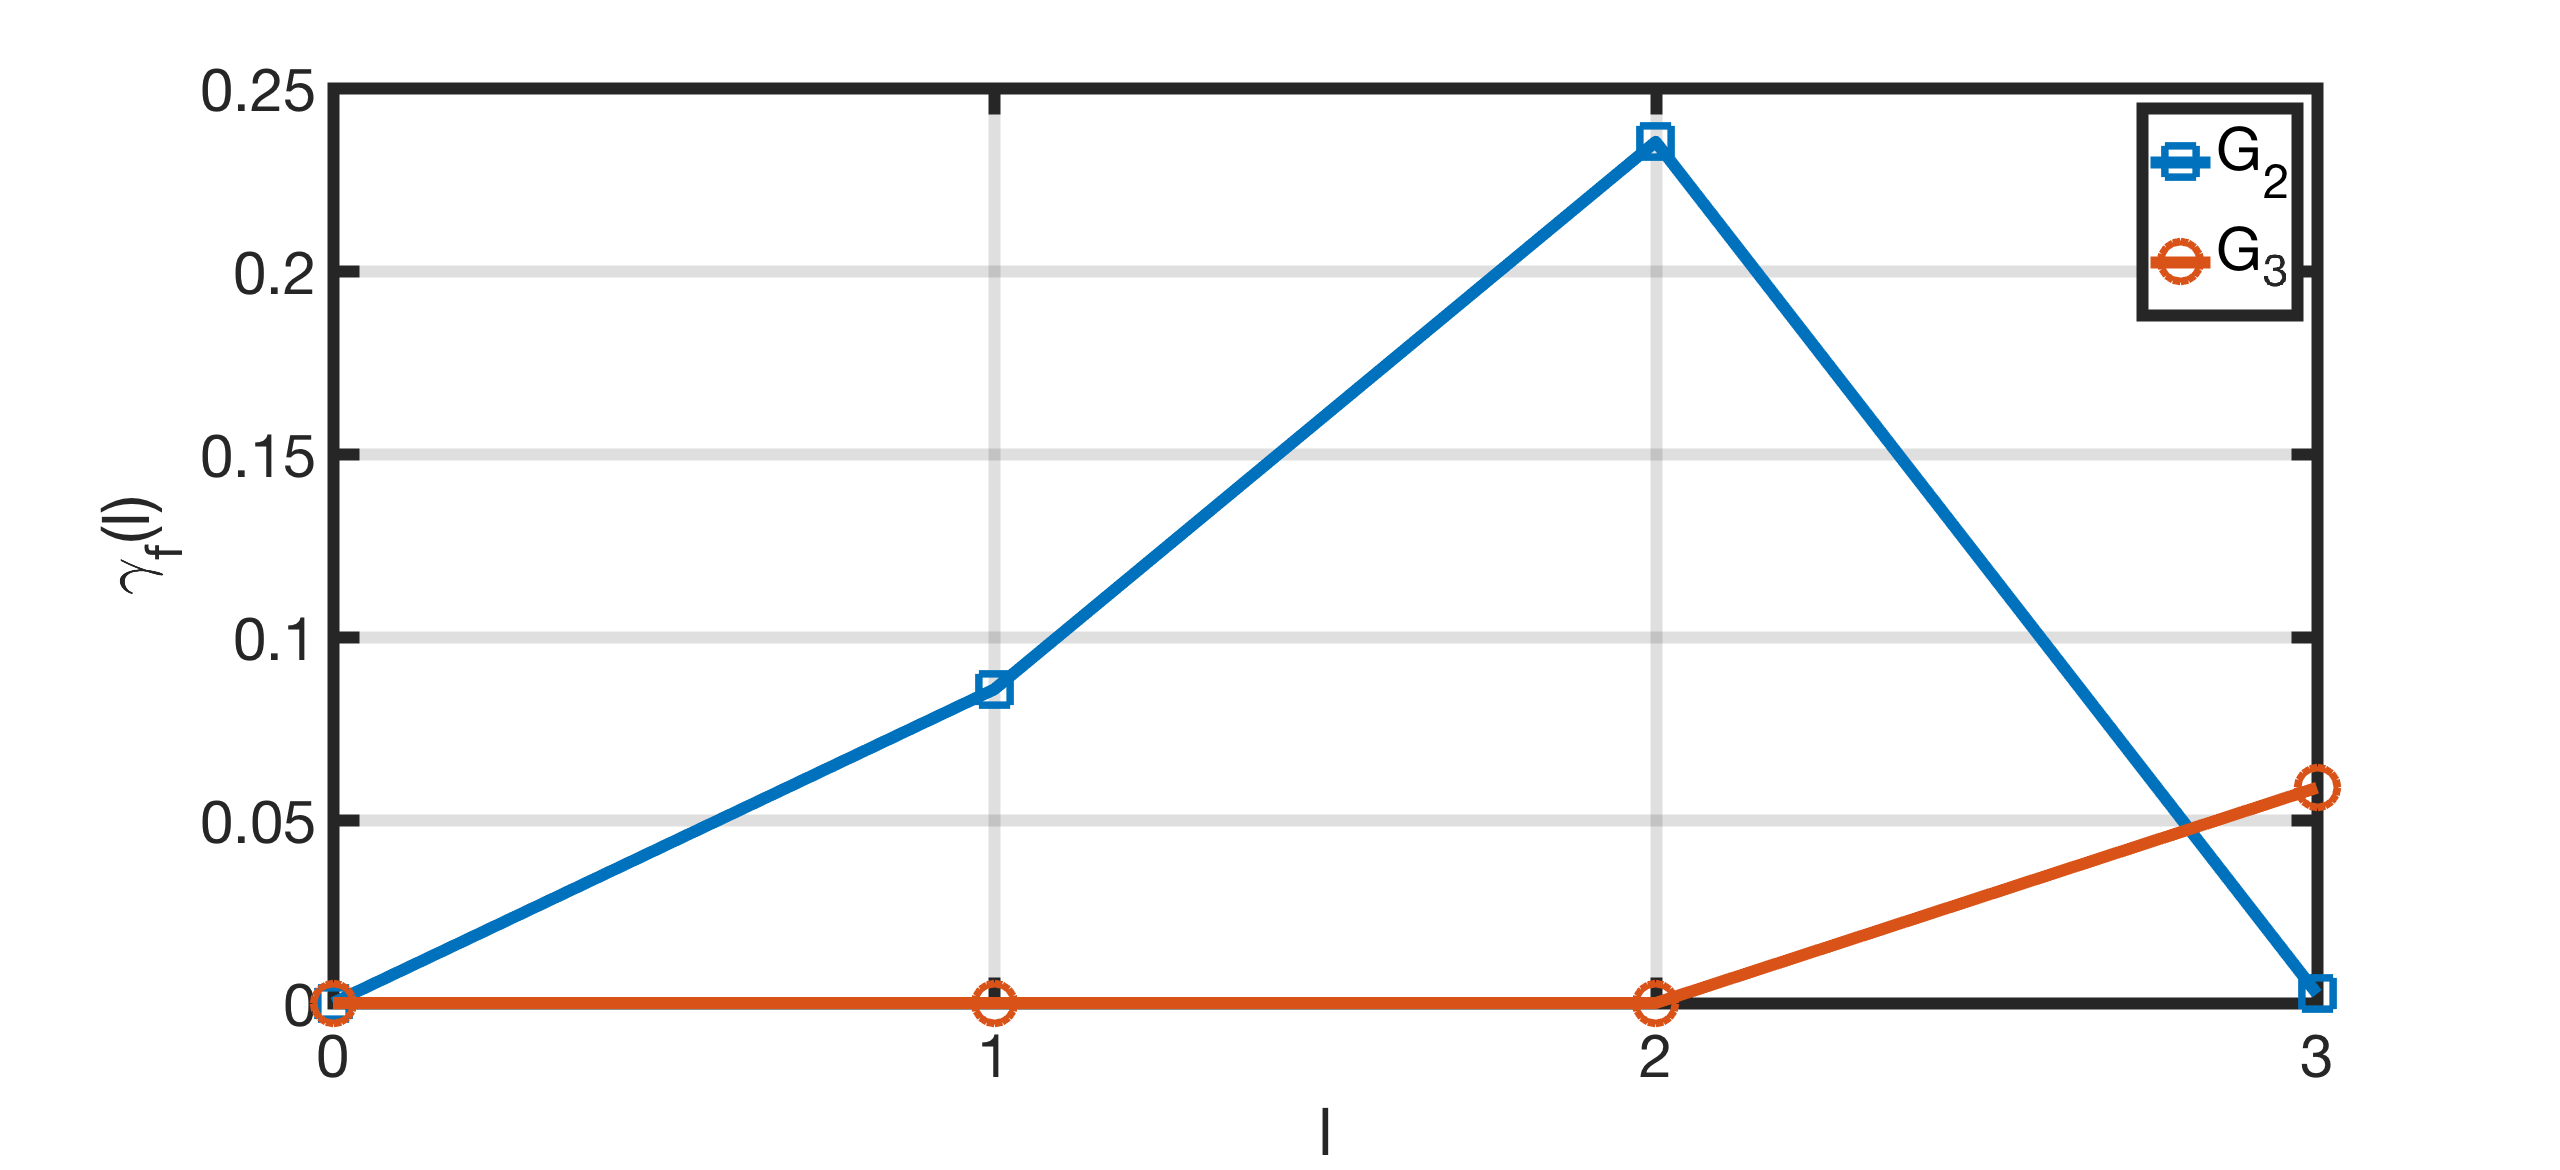
\includegraphics[width= 4in] {figures/new_graph.png}
		\label{fig:distribution2}
	}
	\caption{Anomaly index of $\mathbf{G_2}$ and $\mathbf{G_3}$.}
	\label{fig:new_graph}
\end{figure}




Figure \ref{fig:g1_gamma} plots the anomaly Index $\gamma_f(l)$ of $f_1$ on graph $\mathbf{G_1}$, where $f_1=[2,3,4,3,2,1]$. The six markers on the dashed blue are the six eigenvalues of $\mathbf{G}$. The yellow line is $|\hat{f}(l)|$, and the pink line is the anomaly Index, $\gamma_f(l)$ for frequency $\chi_l$. Because $\gamma_f(l)$ depends on both $\lambda_l$ and its power $\hat{f}^2(l)$, in the yellow line, even though $\chi_0$ has the strongest power,  while its deviation $\lambda_0 = 0$, thus  $\gamma_f(0)=0$. On the other hand, $\chi_5$ has the largest deviation; but its power $|\hat{f}(5)|^2$ is small, which makes $\gamma_f(5)$ is also small. Considering $\chi_4$ has a high deviation (eigenvalue) and a strong power of frequency, thus $\chi_4$  has the largest anomaly Index index. To compare the influence of different $f$ on anomaly index, we show an example in Fig \ref{fig:same_graph}. Set $f_1=[2,3,4,3,2,1]$ and $f_2=[2,2,-3,4,3,1]$, we plot their anomaly index $\gamma_{f}$ and energy $|\hat{f}(l)|$ respectively.
%For comparison, we plot both anomaly index and $|\hat{f}(l)|$ for $f_1$ and $f_2$  on $\mathbf{G_1}$, as shown in Fig \ref{fig:same_graph}, where $f_2=[2,3,4,3,2,1]$.
The light blue color stands for anomaly index, and yellow stands for $|\hat{f}(l)|$. The solid line stands for $f_1$, and dashed line stands for $f_2$. As we can see, for high frequency $\chi_l$, $f_1$ has a larger power than $f_2$, and hence a higher anomaly Index than $f_2$, where $\gamma_{f_1}=0.905$ and $\gamma_{f_2}=0.073$. This is consistent with that $f_1$ has larger deviations than $f_2$.

 As we discussed before, anomaly index depends on graph structure and $f$. Shown in \ref{fig:same_graph}, different $f$ might have very different anomaly index because the power of $\chi_l$ distribution is different. Similarly, even same signal $f$ on two different graphs might have very different anomaly index. Fig \ref{fig:f_on_g} shows two graphs with the same $f=[1,2,5,2]$. Fig~\ref{fig:new_graph} illustrates the anomaly index of $f$ on $\mathbf{G_2}$ and $\mathbf{G_3}$, where $\gamma_{f}(\mathbf{G_2})=0.073$ and $\gamma_{f}(\mathbf{G_3})=0.235$. {This is because in $\mathbf{G_3}$ there is not edge connecting $v_2$ and $v_3$, the different between $f(2)$ and $f(3)$ is not considered as anomaly.}


{\textbf{Remarks:}}
In this subsection, we introduce the anomaly index $\gamma_f(l;\mathbf{G})$ to measure the anomaly of $\chi_l$ in $f$ defined on $\mathbf{G}$ by combing the spectrum structure of $\mathbf{G}$ and $f$. $\gamma_f(l;\mathbf{G})$ depends on two parts: (1) the eigenvalue which reflects the deviations of $\chi_l$; (2) the $|\hat{f}(l)|^2$  which represents the power of $\chi_l$ in $f$. $\gamma_f(l;\mathbf{G})$ reflects the anomaly index of $\chi_l$ and not about the vertex $v_l$. We use the maximal value of $\gamma_f(l;\mathbf{G})$ to define the anomaly index of $f$ defined on $\mathbf{G}$, and it denotes the global anomaly index of $f$ on $\mathbf{G}$.


\subsection{Graph Wavelets}
\label{sec:graph_wavelet}
Classic wavelet is called mathematical microscope because of its capability of showing signal abnormality with different scales.
In the case of complex networks, graph wavelets render the graph with good localization properties both in frequency and vertex (i.e. spatial) domains. Their scaling property allows us to zoom in/out of the underlying structure of the graph.

%It is useful to analyze $f$ by taking into account the intrinsic geometric structure of the graph $\mathbf{G}$. In order to identify and exploit structure of  $f\in \mathbb{R}^N$, the spectral graph $\sigma({\mathcal{L}}):=\{\chi_l\}_{l=0}^{N-1}$ can be used as a dictionary of atoms~\cite{shuman_ACHA_2013}. Thus, $f$ can be decomposed as a linear combination of $\{\chi_l\}_{l=0}^{N-1}$ as
%\begin{equation}
%\label{eq:graph_fourier}
%f(n)= \sum\limits_{l=0}^{N-1}\hat{f}(l)\chi_l(n)
%\end{equation}
%, where
%\begin{equation}
%\label{eq:graph_fourier1}
%\hat{f}(l):= \sum\limits_{n=0}^{N-1}\chi^*_l(n)f(n)
%\end{equation}
%$\chi_l$ is called the Fourier frequency of $f(n)$ based on the graph $\mathbf{G}$, and $\hat{f}(l)$ is the corresponding Fourier coefficient.
%Equation~\ref{eq:graph_fourier1} and Equation~\ref{eq:graph_fourier} are called Fourier transform and inverse Fourier transform, respectively.
%Equation~\ref{eq:graph_fourier1} gives a clear representation of the Fourier components in $f(n)$.

Recall from Equation~\ref{eq:Graph_Fourier_Transform1}, the anomaly pattern $\hat{f}(l)$ presents the anomaly components of $f$ from the whole graph prospective. However, information concerning the vertex-location can not be identified from the Fourier transform. To address this issue, Hammond et al.~\cite{hammond2011wavelets} proposed constructing wavelet transforms of functions over the vertices using weighted graphs, described in the following steps:

\begin{enumerate}
\item Define a continuous generating kernel functions $g(x)$ on $\mathbb{R}^+$;
\item Then, select a central vertex $a \in {V}$ and scale $s$, set the frequency coefficients as $g(s\lambda_l)\chi^*_l(a)$ for each frequency component $\chi_l$;
\item Finally, sum up all those frequency components $\chi_l$.
\end{enumerate}
In this way, the graph wavelet at central vertex $a$ is constructed as:
\begin{equation}
\label{eq:graphwaveletdefinition}
\psi_{s,a}(n) = \sum\limits_{l=0}^{N-1}g(s\lambda_l)\chi_l^*(a)\chi_l(n)
\end{equation}
%After setting up the graph wavelet, the wavelet coefficients for $f$ can be defined as
%\begin{equation}
%\label{eq:graph_graphwavelet}
%W_f(s,a)=<\psi_{s,a}, f>=\sum\limits_{l=0}^{N-1}g(s\lambda_l)\hat{f}(a)\chi_l(n)
%\end{equation}
%\paragraph{\textbf{Properties}}


Similar to classical wavelets, graph wavelets provide following three properties, which are presented in detail in~\cite{hammond2011wavelets}.
 \begin{enumerate}
 \item \textbf{Reconstruction.}
 When generating the kernel function $g(x)$ satisfies the admissibility condition and $g(0)=0$,  $f(n)$ can be reconstructed by the wavelet coefficients.
\item \textbf{Discretization and Wavelet Frames} For practical applications, scale $s$ of graph wavelet $\psi_{s,a}$ should be sampled with a finite number of scales. Given a real valued function $h(x)$, satisfying
\begin{equation}
\hat{h}(\omega) = \sqrt{\int_\omega^\infty\frac{|\hat{g}(\omega')|^2}{\omega'}d{\omega'} }
\end{equation}
, where $\hat{g}$ and $\hat{h}$ are the classical Fourier transform of $g(x)$ and $h(x)$, the scaling function $\phi_{a}(n)$ can be generated as:
\begin{equation}
\label{eq:graphscaledefinition}
\phi_{a}(n) = \sum\limits_{l=0}^{N-1}h(\lambda_l)\chi_l^*(a)\chi_l(n)
\end{equation}
%Accordingly, the scaling coefficients are defined as
%\begin{equation}
%S_f(a)=<\phi_a,f>
%\end{equation}
Using scale set $\Theta:=\{s_j\}_{j=1}^J$, the discretized graph wavelet set $\{\psi_{s_j,a}\}_{j=1}^{J}$ $_{a=0}^{N-1}$, and scaling function set $\{\phi_a\}_{a=0}^{N-1}$ constitute a frame~\cite{hammond2011wavelets}.
So there will be $NJ$ wavelet coefficients in the frame.
According to frame theory~\cite{daubechies1992ten}, $f\in \mathbb{R}^N$ can be reconstructed by a limited number of scaling and graph wavelet coefficients. A detailed algorithm and treatment concerning the choice of $\Theta$ can be found in~\cite{hammond2011wavelets}.


\item \textbf{Localization in vertex domains}. Given a central vertex $v_a$ and its graph wavelet $\psi_{s,a}$, suppose the kernel function $g$ is $K+1$ times continuously differentiable, let $v_n$ be an vertex of $\mathbf{G}$ with $d_G(n,a)>K$, then there exist constants $D$ and $s_0$, such that
\begin{equation}
\label{equ:waveletbound}
\frac{\psi_{s,a}(n)}{||\psi_{s,a}||}\leq Ds_0
\end{equation} for all $s<s_0$ .
$d_G(n,a)$ is the shortest path distance, which is the minimum number of edges in any path that connect vertices $v_n$ and $v_a$~\cite{hammond2011wavelets}. Equation~\ref{equ:waveletbound} shows for any vertex $v_n$ that is far away from center vertex $v_a$ ($d_G(n,a)>K$), its wavelet value $\psi_{s,a}(n)$ is upper bounded by $Ds_0$. In other words, for vertex $v_n$ which is far away form vertex $v_a$, its wavelet value is linearly attenuated by scale $s$. When the scale $s$ is small, their wavelet value will be vanished quickly. Figure~\ref{fig:graphwaveletscale} shows two graph wavelets centered on the same vertex $v_a$, but with two different scales, $\psi_{s_1,a}$ and $\psi_{s_2, a}$, where $s_1<s_2$. The length of the black bar on each vertex denotes its graph wavelet value. The highlighted areas denote the kernel vertex with larger graph wavelet values.

Figure~\ref{fig:scale3} is $f$'s distribution along each vertex, whose value is denoted as the vertical bar. As we can see, with the graph wavelet pattern of $\psi_{s_2,a}$, $f$ shows a larger value on most of the kernel vertices, and $W_f(s_2,a)$ a large value as well. That also means $\psi_{s_2,a}$ optimally partitions the set $V$ into two distinct groups - kernel and marginal vertices. As shown in Figure~\ref{fig:scale4}, $W_f(s_3,a)$ is where the absenteeism is most significant, and $W_f(s_2,a)$ is  where bursty behavior is observed.
 \end{enumerate}
 
 

\begin{figure*}[t]
	\centering
	\subfigure[wavelet $\psi_{s_1,a}$]{
		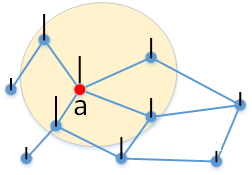
\includegraphics[width=1.4in, height=1.1in] {figures/wavelet1.png}
		\label{fig:scale1}
	}
	\subfigure[wavelet $\psi_{s_2,a}$]{
		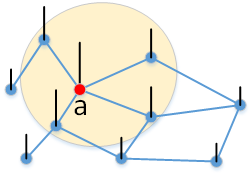
\includegraphics[width=1.4in, height=1.1in] {figures/wavelet2.png}
		\label{fig:scale2}
	}
\subfigure[$f(n)$ vs vertices]{
		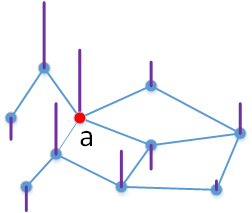
\includegraphics[width=1.4in, height=1.1in] {figures/wavelet3.png}
		\label{fig:scale3}
	}
\subfigure[$W'_f(s,a)$ vs scale $s$]{
		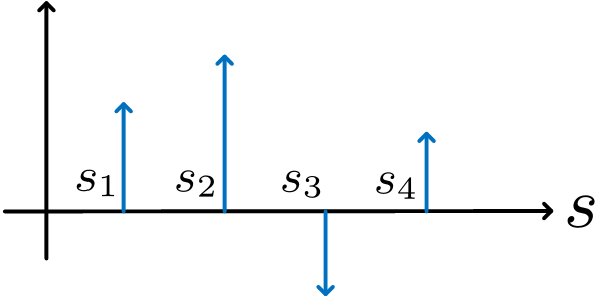
\includegraphics[width=1.5in, height=1.1in] {figures/wavelet4.png}
		\label{fig:scale4}
	}
	\caption{Using graph wavelets for abnormal group identification.}
	\label{fig:graphwaveletscale}
\end{figure*}


% {\textbf{Remarks:}} Essentially, the wavelet frame is generated by kernel function $g(x)$ and scaling function $h(x)$ with $J$ different scales. Those functions are also called filter banks. Figure~\ref{fig:brazil_filter} shows the wavelet filter banks for Brazil graph which we will mention in the experiment part.

% \begin{figure}[h]
% 	\centering
%     {
% 		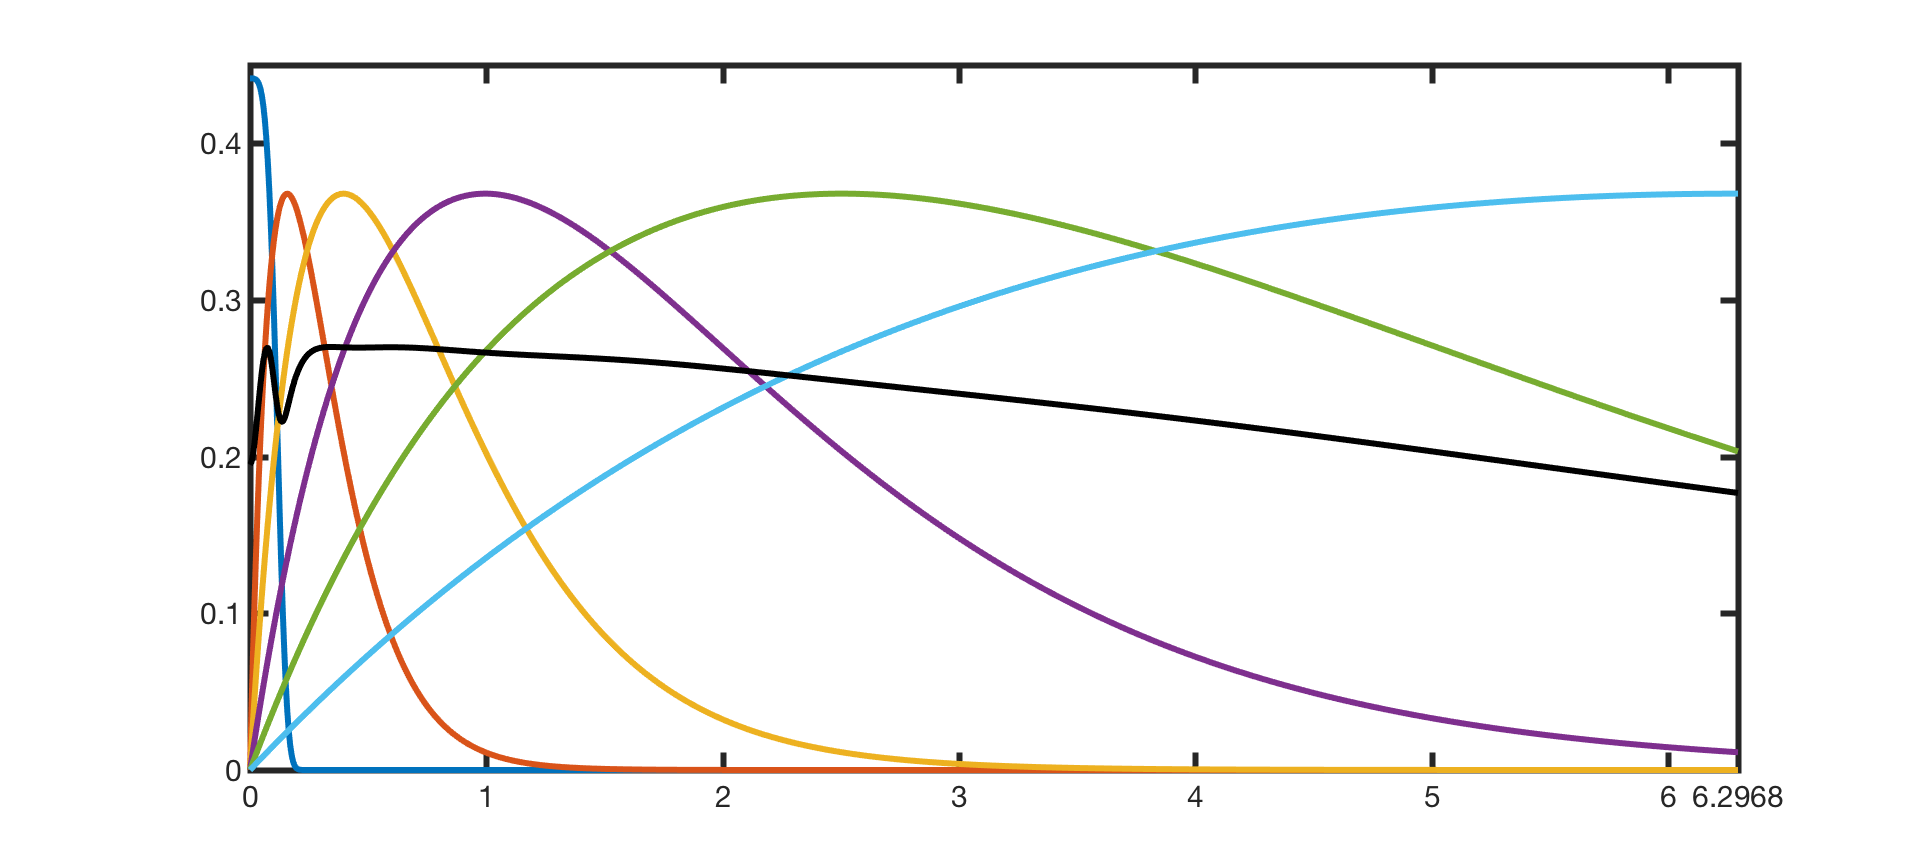
\includegraphics[width= 3.2in] {figures/brazil_filter.png}
% 		\label{fig:distribution2}
% 	}
% 	\caption{Wavelet filter banks for Brazil graph.}
% 	\label{fig:brazil_filter}
% \end{figure}



\subsection{Group Anomaly Detection via graph wavelet}
\label{sec:Group_Anomaly_Detection_via_graph_wavelet}
For a center node $a$, its kernel vertices denoted by $\mathcal{K}(a)$, is defined a set of vertices such that $d_G(n,a)\leq K$. All the other vertices are called as marginal vertices. One thing need to mention is that for different scale $s$, the $\mathcal{K}({a})$ is the same.
According to Equation~\ref{equ:waveletbound}, when $s$ is small, the weights of the marginal vertices are severely attenuated.
Essentially, $W_f(s,a)$ is equivalent to the sum of $f$ with large weights on kernel vertices, and small weights on marginal vertices.
%, and can also be treated as a similarity between $f$ and $\psi'_{s,a}$.
When $f$ is of uniformly large negative/positive value on kernel vertices, then $W_f(s,a)$ will be a large negative/positive value with scale $s$.
We call the wavelets with minimal and maximal $W_f(s,a)$ absenteeism wavelet and burst wavelet, respectively.


The localization property of graph wavelet makes it appropriate for group anomaly detection since it automatically identifies the kernel vertices from $V$.  These kernel vertices form a compact subset since each one of them is close to the same center vertex $v_a$, which avoids the compactness constrain condition, thus its complexity is greatly reduced. We propose our anomaly Group detection based on graph wavelet in Algorithm~\ref{algo:event_detection1}.



\begin{algorithm}[ht]
\centering
\captionsetup{font=scriptsize}
\caption{Anomaly Group Detection Using Graph Wavelet}
{\footnotesize \begin{algorithmic}[1]
\STATE {\bf Input:} graph and absenteeism score vector $\mathbf{G}(V,E;f^l)$ at time interval $l$, and wavelet threshold $\omega_{th}$.
\STATE {\bf Output:} anomaly burst group set $\mathcal{I}^{bur}$ and absenteeism group set $\mathcal{I}^{abs}$.	
\STATE{compute the spectral $\sigma{(\mathcal{L})}$ of graph $\mathbf{G}$};
\STATE{set the graph wavelets $\psi_{s,a}(n)$ and scales set $\{s_j\}_{j=1}^J$ for all $a\in V$};
\FORALL {$v_n\in V$ and $s_j \in \{s_j\}_{j=1}^J$}
	    \STATE{compute $W_f(s_j, a)$};
		\IF {$W_f(s_j, a) \ge \omega_{th}$}
		    \STATE{add group $\mathcal{K}(s_j,v_n)$ to $\mathcal{I}^{bur}$}
	    \ENDIF
	
		\IF {$W_f(s_j, a)\le -1*\omega_{th}$}
		    \STATE{add group $\mathcal{K}(s_j,v_n)$ to $\mathcal{I}^{abs}$}
	    \ENDIF	
	
\ENDFOR	
\RETURN {anomaly burst group $\mathcal{I}^{bur}$ and absenteeism group set $\mathcal{I}^{abs}$.}
\end{algorithmic}}
\label{algo:event_detection1}
\end{algorithm}


{\textbf{Remarks:}}
\begin{enumerate}
\item As graph wavelet and scaling functions form a frame, the function $f$ can be reconstructed by their coefficients.
As long as the scale level $J$ is high enough, $f$ can be well decomposed into the frame basis. Thus, using graph wavelets to exploit structure of functions defined on graphs is much more reasonable.
\item Graph wavelet transforms select vertices that are close to the central vertex $v_a$, and attenuate the impact of other marginal vertices that are far away from $v_a$.
Unlike other conventional methods,  $\psi_{s,a}$ is automatically scalable, and maintains the graph's topological information.
\item The graph wavelet does not introduce any objective functions and constraints. In addition, the scale $\{s_j\}_{j=1}^J$ set is numerically small, and once the eigenvalues and eigenvectors of $\mathbf{G}$ are known, the computation complexity of graph wavelet coefficients is $O(NJ)$, which makes is easily adaptable to wide variety of application scenarios.
\end{enumerate}


\subsection{Group Absenteeism Event Detection}
\label{sec:Group Absenteeism Event Detection}
In our real world, there are various scenarios that causes people's silent on the social media for a certain amount of time. Take Earthquake emergence for example, when earthquake is happening, people hardly get a chance to use social media and even the communication infrastructure are paralyzed, thus it will cause twitter uniformly Absenteeism. Some other examples, like flooding, blackout, and so on. We call this kind of disaster events as Absenteeism Event. When the disaster is over, and people's circumstance recovered, there follows some kind of burst in social media since it's natural for people to comment their recent experience. Usually, the severer of the disaster events, the stronger Absenteeism signal the social media may present when the even is happening, and the stronger burst signal will follow after that.

We propose a novel two-pass absenteeism based event detection algorithm. The underlying rationale of this algorithm is based on the following concepts.
\begin{enumerate}
\item As discussed in section~\ref{sec:graph_wavelet}, distribution of $f$ can be well reconstructed by the $J$ scaling and $NJ$ wavelet coefficients. Each of those normalized wavelet coefficients $W_f(s,a)$ represents a distribution pattern of $f$ on $\mathbf{G}$.
It is equivalent to saying that $\psi_{s,a}$ represents a special distribution pattern, which shares a large and uniform value around the central vertex with scale $s$.
\item When a significant event occurs, preceded by group absenteeism behavior in social networks, such as a severe earthquake, it is likely to be succeeded by a spike or burst in online user activity.
With this observation, we can represent an absenteeism behavioral pattern as $\psi_{s_l,a_l}$ at time $l$ centering at vertex $v_{a_l}$, and a burst related pattern as $\psi_{s_{\tau,a_\tau}}$ at time $\tau$ centering at vertex $v_{a_\tau}$. We assume the burst pattern happens within the time window size of $L$ after absenteeism pattern is identified. Further, a notion of response time can represented using the time difference $t_{rsp}=\tau-l$.
\item Both absenteeism and burst signal must show a strong correlation, especially if they occur in close proximity spatially and temporally.
%For instance, taking the power-cut-off for instance, usually only people who live in the affected area will ``yield at " this event a lot because it brings inconvenience to their life. However, people who live outside of the affected areas would hardly mention this event. Thus, to measure the correlation between absenteeism pattern and burst pattern is proposed as:
\begin{equation}
\label{eq:eventsimilarity}
\rho(\mathcal{K},\mathcal{K'}) = \frac{|\mathcal{K}\cap\mathcal{K'}|}{|\mathcal{K}|\cdot|\mathcal{K'}|}
\end{equation}
Based on these concepts, the higher the correlation, the higher probability that burst patterns is caused by the preceding group absenteeism. When $\rho$ is above the threshold (threshold is set at 0.5), we infer that an event occurred and that it evolved on social networks into distinct phases: first group absenteeism, followed by a spike or burst in user activity.
\end{enumerate}



\begin{algorithm}[t]
\centering
\captionsetup{font=scriptsize}
\caption{Two-Pass Absenteeism Event Detection}
{\footnotesize \begin{algorithmic}[1]
\STATE {\bf Input:} graph and absenteeism score vector $\mathbf{G}(V,E;f^l)$ at time interval $l$, and time window size $L$.
\STATE {\bf Output:} absenteeism event set $\mathcal{E}$.	
\STATE{compute burst group set $\mathcal{I}^{bur}$ by algorithm~\ref{algo:event_detection1}};
		    	\FORALL {$\tau$ from $l+1$ to $l+L$}
		    	    \STATE{compute absenteeism group set $\mathcal{I}^{abs}$ by algorithm~\ref{algo:event_detection1}};
		    	    \FORALL {$\mathcal{K}(a)\in \mathcal{I}^{bur}$ and $\mathcal{K}(b)\in \mathcal{I}^{abs}$}
		
		    	    \STATE{compute $W_{f^\tau}(s_k, b)$};
		    	    		
		    	    		    \IF {$\rho(\mathcal{K},\mathcal{K'})\ge \rho_{th}$}
		    	    		    \STATE{add absenteeism event $e\{a,b,\tau\}$ to $\mathcal{E}$}
		    	    	    	\ENDIF

                   \ENDFOR

	            \ENDFOR	
		


\RETURN {absenteeism event set $\mathcal{E}$}.
\end{algorithmic}}
\label{algo:event_detection}
\end{algorithm}
In summary, the two-pass absenteeism event detection can be summarized as shown in Algorithm~\ref{algo:event_detection}. Because the computation of the graph spectral graph $\sigma(L)$ is a one-time computation, the two-pass algorithm has $O(NJ)$ complexity.
\begin{enumerate}
\item Compute $\mathbf{G}$'s spectral graph $\sigma(L)$. Because $\sigma(L)$ is independent of the time interval, it is computed only once and can be solved by classical matrix factorization methods.
\item Set scale set $\{s_j\}_{j=1}^J$ according to algorithms in~\cite{hammond2011wavelets}, and compute the $NJ$ normalized graph wavelet coefficients $W'_f(s_j, a)$ at current time interval $l$.
\item Identify the most negative $W'_f(s_l, a_l)$, and determine the corresponding $\psi_{s_l,a_l}$ as the absenteeism pattern.
\item For all the time interval $\tau$ from $l+1$ to $l+L$, compute all the $W'_f(s_j, a)$, detect the most positive one and identify the corresponding graph wavelet $\psi_{s_\tau,a_\tau}$ as the burst pattern at time $\tau$, and the correlation score $\rho_{\tau}$ between absenteeism pattern $\psi_{s_l,a_l}$ and burst pattern $\psi_{s_\tau,a_\tau}$.
\item Detect the largest $\rho_{\tau}$ as $\rho_{max}$; return $\rho_{max}$ and response time $t_{rsp}$.
\end{enumerate}


\begin{figure}[h]
	\centering
    {
		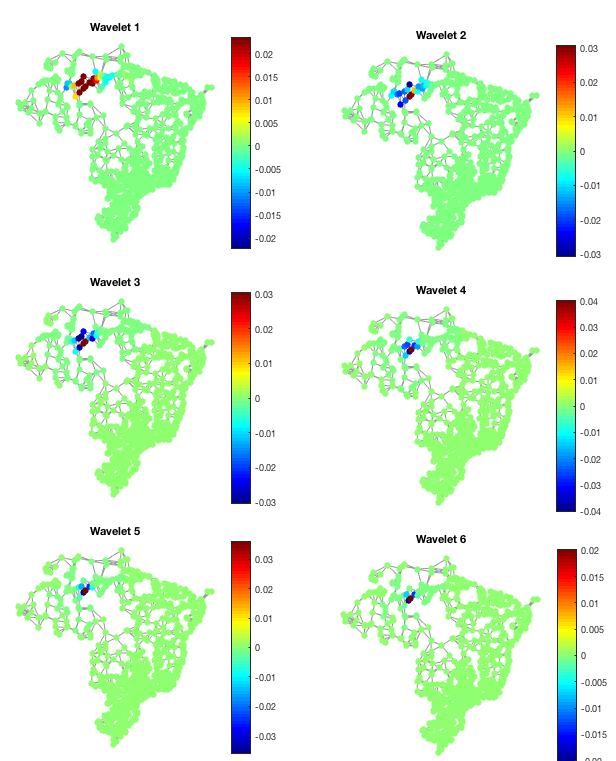
\includegraphics[width= 3.3in] {figures/brazil_wavelet_small.png}
	}
	\caption{Graph Wavelets with center city $v_{83}$.}
	\label{fig:brazil_wavelet_small}
\end{figure}




\begin{figure}[th]
	\centering
	\subfigure[wavelet $\psi_{s_1,a}$]{
		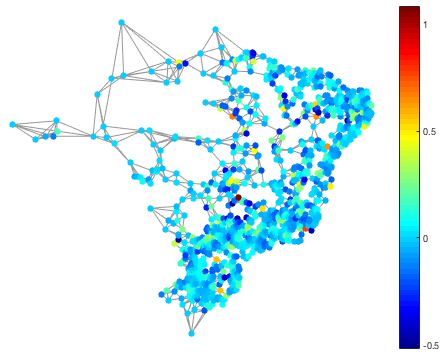
\includegraphics[width=2in] {figures/Brazil_W_coeff_date31_s3.png}
		\label{fig:Brazil_W_coeff_date31_s3}
	}
	\subfigure[wavelet $\psi_{s_2,a}$]{
		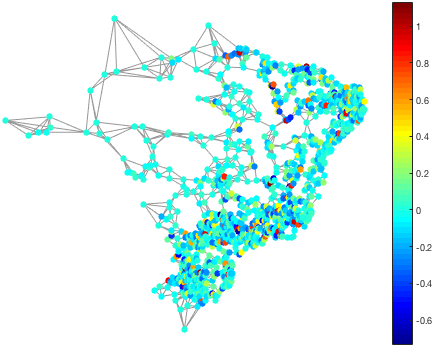
\includegraphics[width=2in] {figures/Brazil_W_coeff_date31_s5.png}
		\label{fig:Brazil_W_coeff_date31_s5}
	}
	\caption{Graph Wavelet coefficient with scale $s_3$ and $s_5$.}
	\label{fig:graphwaveletcoefficient}
\end{figure}


